\section{VQ-VAE}
\label{sec:vqvae}

Vector Quantized Variational Autoencoder (VQ-VAE) \cite{vqvae} is a generative models based on VAE \ref{sec:vae} model with the addition of vector quantization (VQ) (section \ref{subsec:vqvae_vq}) technique. 


\begin{figure}[h]
    \centering
    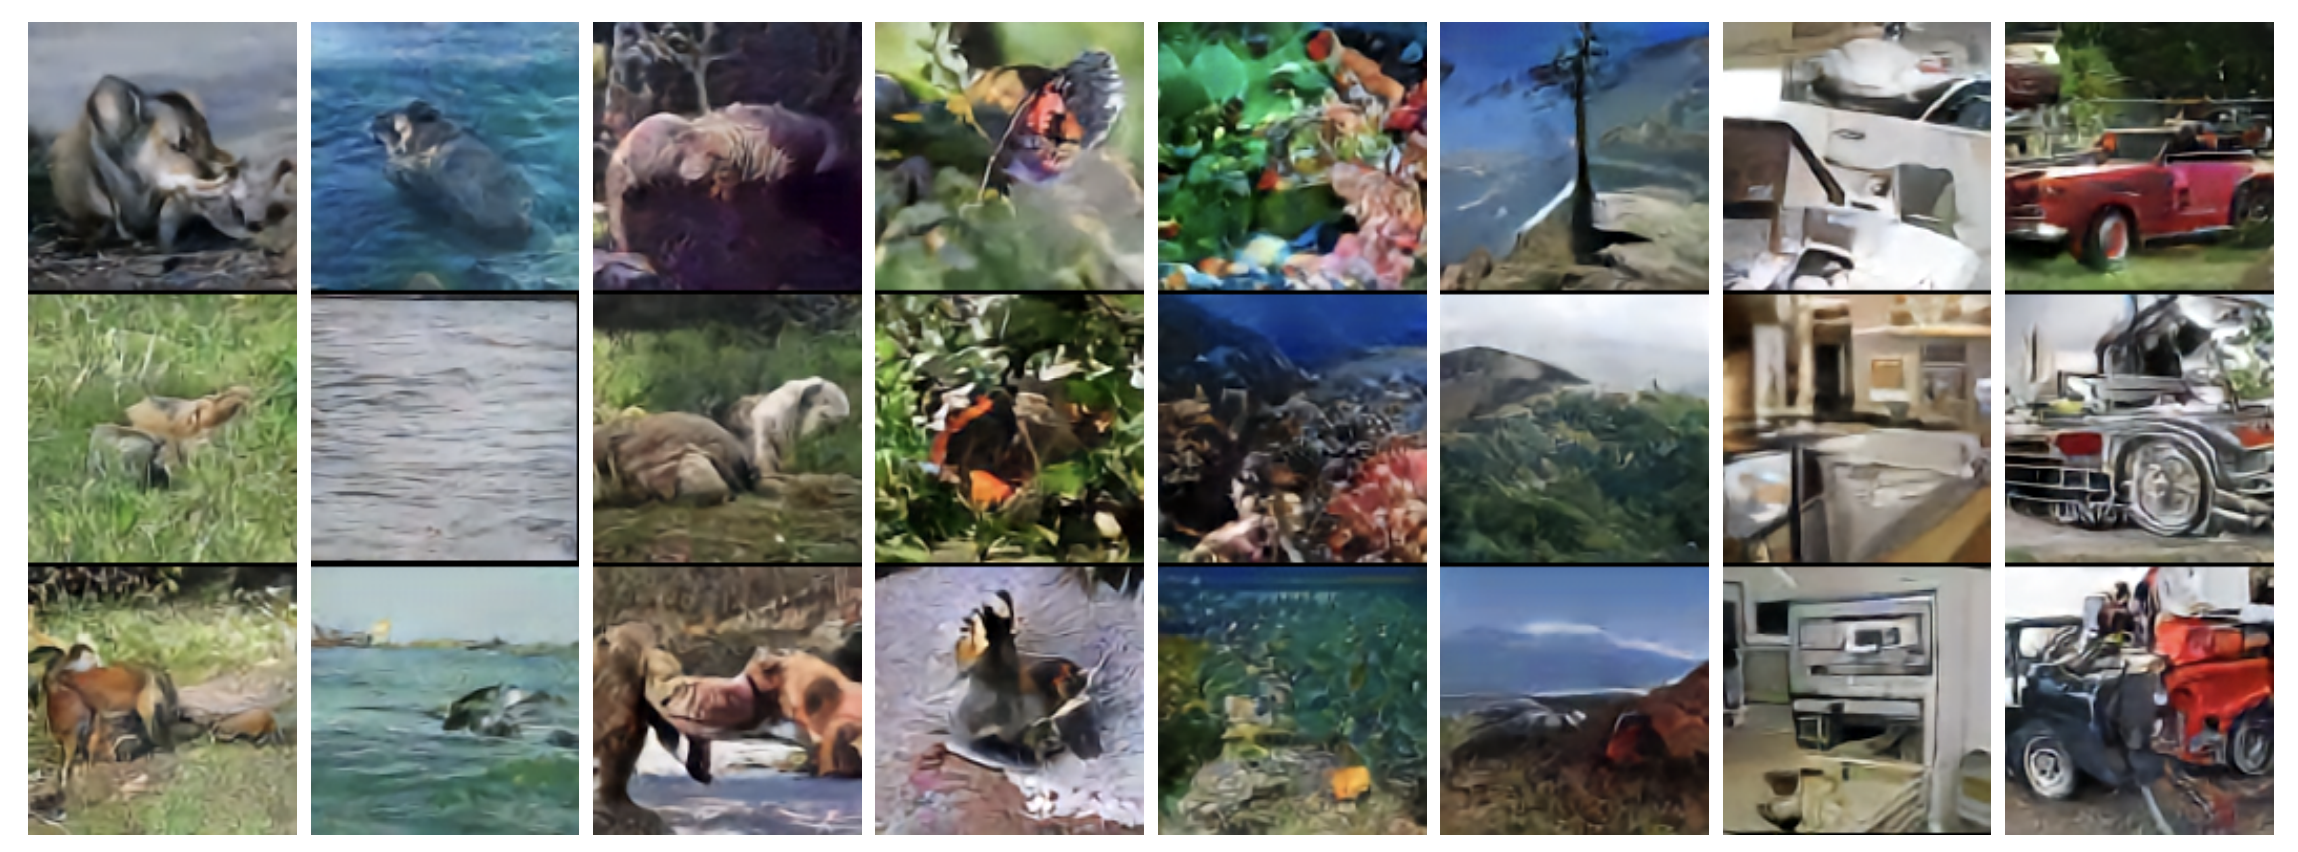
\includegraphics[width=\textwidth]{images/vqvae_samples.png}
    \caption{Samples generated by VQ-VAE model \cite{vqvae}, trained on ImageNet dataset. From left to right:  kit fox, gray whale, brown bear, admiral (butterfly), coral reef, alp, microwave, pickup.}
\end{figure}










\subsection{Vector Quantization}
\label{subsec:vqvae_vq}

Vector quantization (VQ) is a technique used to discretize continuous data. In other words this technique allows the representation of a set of vectors using smaller set of representative vectors called codebook. In the context of VQ-VAE, the continuous latent space $z$ (the embeddings) is mapped into discrete codes vectors. In a continuous latent space, the amount of possibilities for a value in the hidden space is infinite, which makes it difficult for the model to learn the hidden space efficiently. With a discrete hidden space, learning becomes more efficient because there is a fixed and smaller number of possible values (although in reality it is very large, for example the amount of objects that can be described using language is finite but very large). Furthermore, in reality, images are divided into classes of objects such as cats, people, dogs, etc., and each class has a finite number of variations / possibilities, which is better suited to a discrete latent vectors. VQ is a form of lossy compression, where the goal is to reduce the amount of data while preserving important features.

\begin{figure}[h]
    \centering
    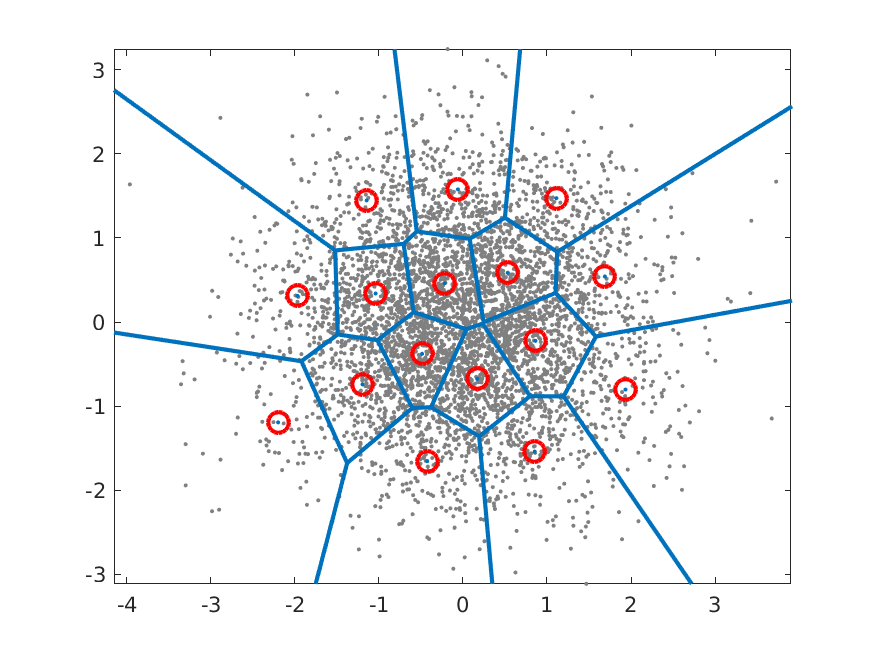
\includegraphics[scale=0.5]{images/vq_visualization.png}
    \caption{Illustration of vector quantization: discrete clustering of the 2D latent space \cite{vq_visualization_website}. The grey dots are embeddings of the continous latent space, and the red dots are the code vectors from the codebook. In this case, the codebook size is 16.}
    \label{figure:vq_visualization}
\end{figure}

In the VQ-VAE model, after the input passes through the encoder (which results in embeddings - which are the hidden representation of the input), the embeddings are replaced by the closest vector from the codebook (by minimizing distance between vectors, usually Euclidean distance). This operation allows the model to learn clusters of similar embeddings, which can be used to generate new samples. In other words, the input vectors are partitioned into clusters and each cluster is represented by a codebook vector (code vector) (see eq. \ref{eq:vq_onehot}). These code vectors are then passed through the decoder to generate the output.

\begin{equation}
    \label{eq:vq_onehot}
    q(z=k|x) = \begin{cases}
        1 & \text{if } \text{for } k=\text{argmin}_j \Vert z_e(x) - e_j \Vert_2 \\
        0 & \text{otherwise}
    \end{cases}
\end{equation}

Equation \ref{eq:vq_onehot} shows the one-hot representation of the posterior categorical distribution. One-hot means each vector is categorically 0 or 1. In other words, each embedding is replaced by the (single) closest code vector from the codebook. The Euclidean distance calculation is shown in listing \ref{lst:vqvae_distance}.


\subsection{Architecture}

\begin{figure}[h]
    \centering
    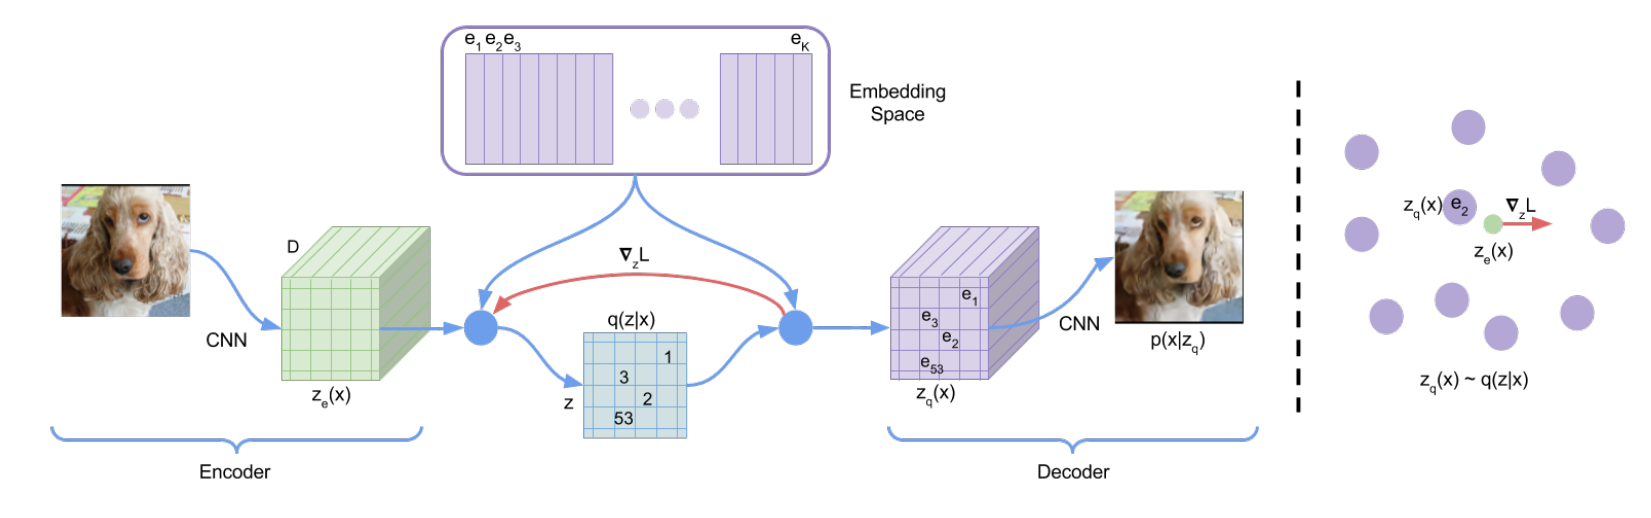
\includegraphics[width=\textwidth]{images/vqvae_architecture.png}
    \caption{VQ-VAE architecture \cite{vqvae}.}
    \label{fig:vqvae_architecture}
\end{figure}

The architecture of VQ-VAE is shown in figure \ref{fig:vqvae_architecture}. The model is similar in structure to VAE but with the addition of vector quantization component (the middle part of the figure), which consists the codebook and CNN layers are used in the encoder decoder networks.

The encoder first maps the input $x$ to a continuous latent space $z_e$ using CNN layers. The embeddings $z_e$ are then quantized to the nearest code vector in the codebook, resulting in the quantized embeddings $z_q$. 

\subsection{Training}



The codebook is learned during training, and the embeddings are quantized to the nearest code vector in the codebook. The codebook is learned by minimizing the loss function:

\begin{equation}
    \mathcal{L}_{\text{VQ}} = || \text{sg}[z_e] - z_q ||_2^2 + \beta || \text{sg}[z_q] - z_e ||_2^2
\label{eq:vq_loss}
\end{equation}

where $z_e$ is the encoder output, $z_q$ is the quantized output, $\text{sg}[\cdot]$ is the stop gradient operation (which prevents gradients from flowing through the quantization operation), and $\beta$ is a hyperparameter that controls the weighting of the two terms in the loss function. The first term in the loss function is the quantization loss, which measures the distance between the encoder output and the quantized output. The second term is the commitment loss, which measures the distance between the quantized output and the encoder output. The commitment loss encourages the model to use the codebook, and prevents the model from ignoring the quantization operation.

Finding the nearest code vector in the codebook is given by equation \ref{eq:quantization} (from the original paper \cite{vqvae}), where $z_e(x)$ is the output of the encoder. The quantizied embeddings are the indecies of the codebook, and not the vectors themselves. The reason is that learning indencies is easier than learning the code vectors, which significantly reduces the number of of parameters in the model. Less computation is needed to find the nearest code vector in the codebook, because the codebook is fixed and the indecies are learned.

\begin{equation}
    \label{eq:quantization}
    z_q(x)=e_k, \text{  where } k = \text{argmin}_j || z_e(x) - e_j ||_2
\end{equation}

In the implementation of the quantisizer module of the VQ-VAE paper, the codebook vectors are initialized using uniform distribution between $-1/n_e$ and $1/n_e$, where $n_e$ is the number of embeddings and $e_d$ is the dimension of the codebook vectors (see listing \ref{lst:vq_codebook}).

Finally, the loss function of the VQ-VAE is given by:

\begin{equation}
    \mathcal{L}_\text{VQ-VAE} = \text{log } p(x|z_q(x)) + \Vert \text{sg}[z_e(x)] - e \Vert_2^2 + \beta \Vert z_e(x) - \text{sg}[e] \Vert_2^2
    \label{eq:vqvae_loss}
\end{equation}
    
    where the first term is the reconstruction loss (MSE), the second term is the quantization loss, and the third term is the commitment loss. The decoder optimizes the first loss term only, the encoder optimizes the first and last loss terms, and the embeddings are optimized in the middle term.






\subsection{Streight Through Estimator (STE)}

It is important to note that snapping embeddings to nearest codebook vectors operation is not differentiable (right side of figure \ref{fig:vqvae_architecture}), which means the gradients will always be 0 at the backpropogation \cite{why_round_function_is_not_differentiable}. For this reason, the researchers used the straight-through estimator (STE) to approximate the gradients. The STE is a technique used to approximate the gradients of a non-differentiable function by passing the gradients of the function through the function itself (see listing \ref{lst:vqvae_stop_gradients}) (in other words, they skip the quantization operation in the backward pass).

\subsection{Video Generation Experiment}

% TODO: The sentence: "correctly projected perspecivel" is not clear, need different phrasing.

\begin{figure}[h]
    \centering
    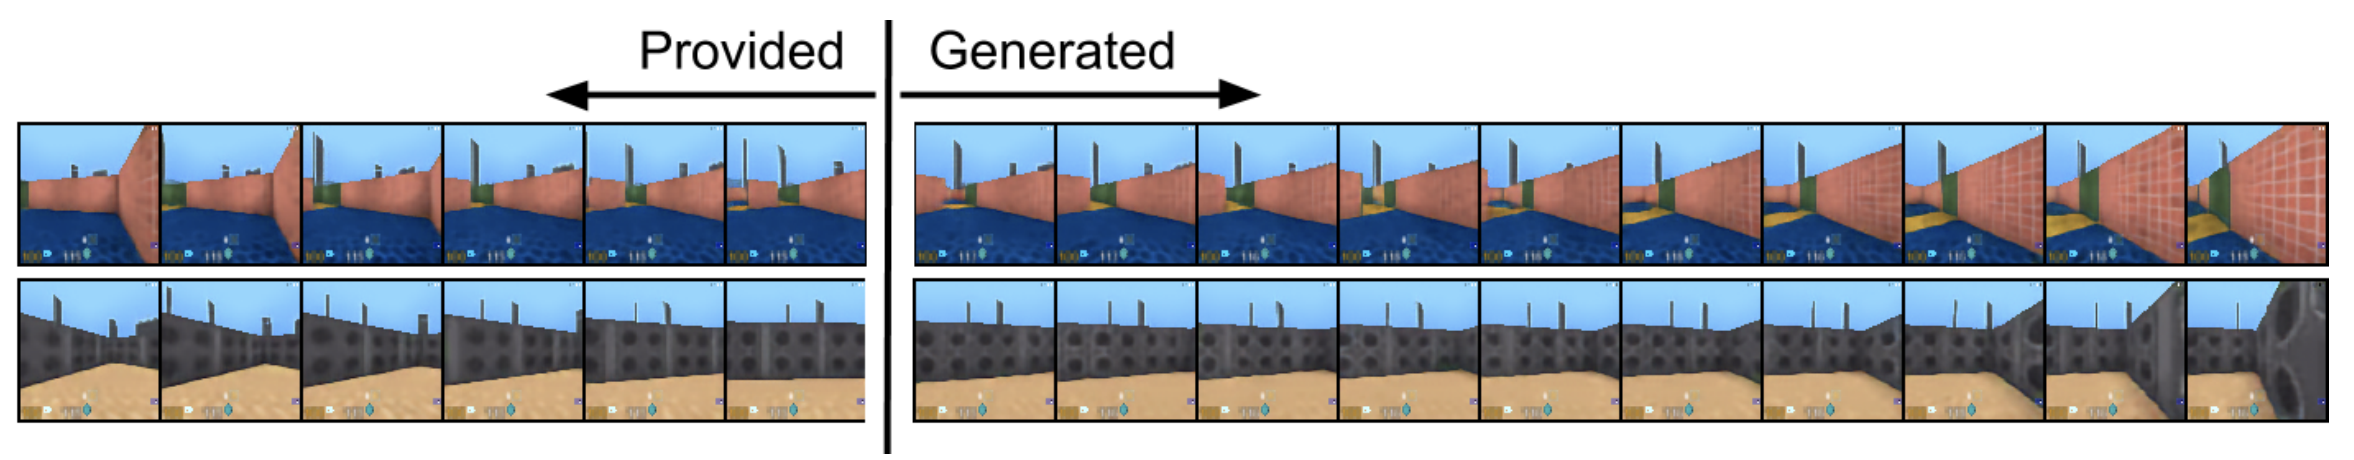
\includegraphics[width=\textwidth]{images/vqvae_video_generation.png}
    \caption{VQ-VAE video generation experiment \cite{vqvae}. Given 6 frames as input, the model predicted the next 10 frames conditioned on the action. Top row is the "move forward" action, bottom row is the "move right" action. In short, the model recognizes the action and creates frames that are correctly projected perspecively.}
    \label{fig:vqvae_video_generation}
\end{figure}

The researchers used the VQ-VAE model to generate videos conditioned on actions (video game controls). In figure \ref{fig:vqvae_video_generation} we can see the results of the video generation experiment. Each image is created by first generating latents and then ingressing into the decoder.
